\section{Analysis}
\label{sec:Analysis}
For this analysis, three different datasets were provided. First, the \texttt{signal\_train.csv} and the \texttt{background\_train.csv} are used to train three different classifiers. For these datasets,
the true values are known so that a proper training can be performed. The \texttt{test.csv} dataset is unlabled and the best perfoming classifier's task is the classification of these data.

\subsection{Data preparation and attribute selection}
The data for the training of the classifiers need to be prepared for this analysis. Therefore, certain non-physical features arising from the Monte Carlo simulations need to be removed. Moreover, all 
features with more than \qty{10}{\percent} non-pyhsical \texttt{NaN} or \texttt{Inf} values are dropped. The remaining rows that contain \texttt{NaN} or \texttt{Inf} values are then deleted. Finally, the
labels with the information whether a measurement is a true signal or true background event is removed from the dataframe. \\
The selection of important features is a crucial part of a multivariate analysis. Here, an mRMR selection (see \autoref{subsec:mRMR}) is performed to find the most relevant features. This is done with the help of the \texttt{python}
extension \texttt{mrmr\_selection} \cite{mrmr} is used. In \autoref{fig:best_features}, the best three features are presentent, whereas less important features are depicted in \autoref{fig:worst_features}.
\begin{figure}
    \centering
    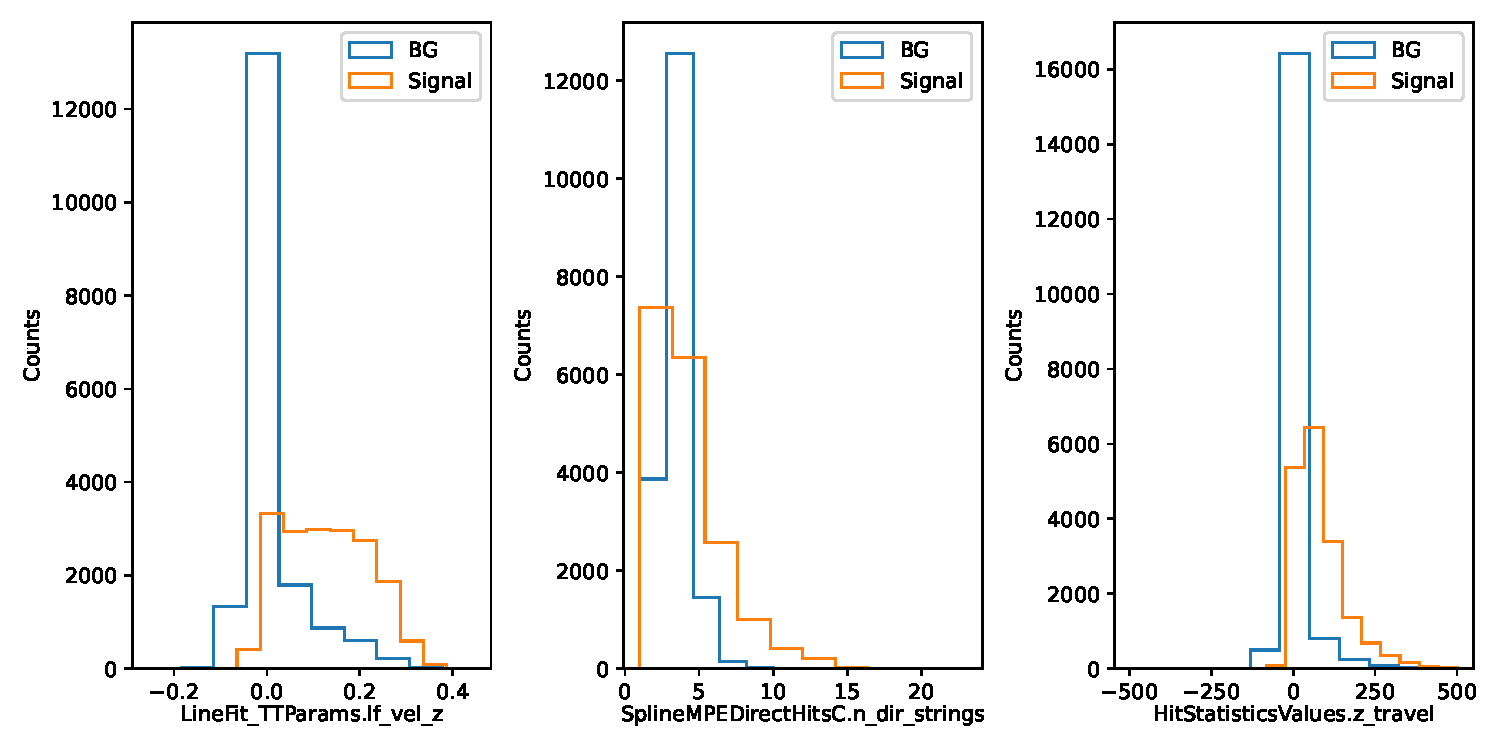
\includegraphics[width=0.9\textwidth]{content/plots/best_3_features.pdf}
    \caption{The best three features determined by the mRMR selection.}
    \label{fig:best_features}
\end{figure}

\begin{figure}
    \centering
    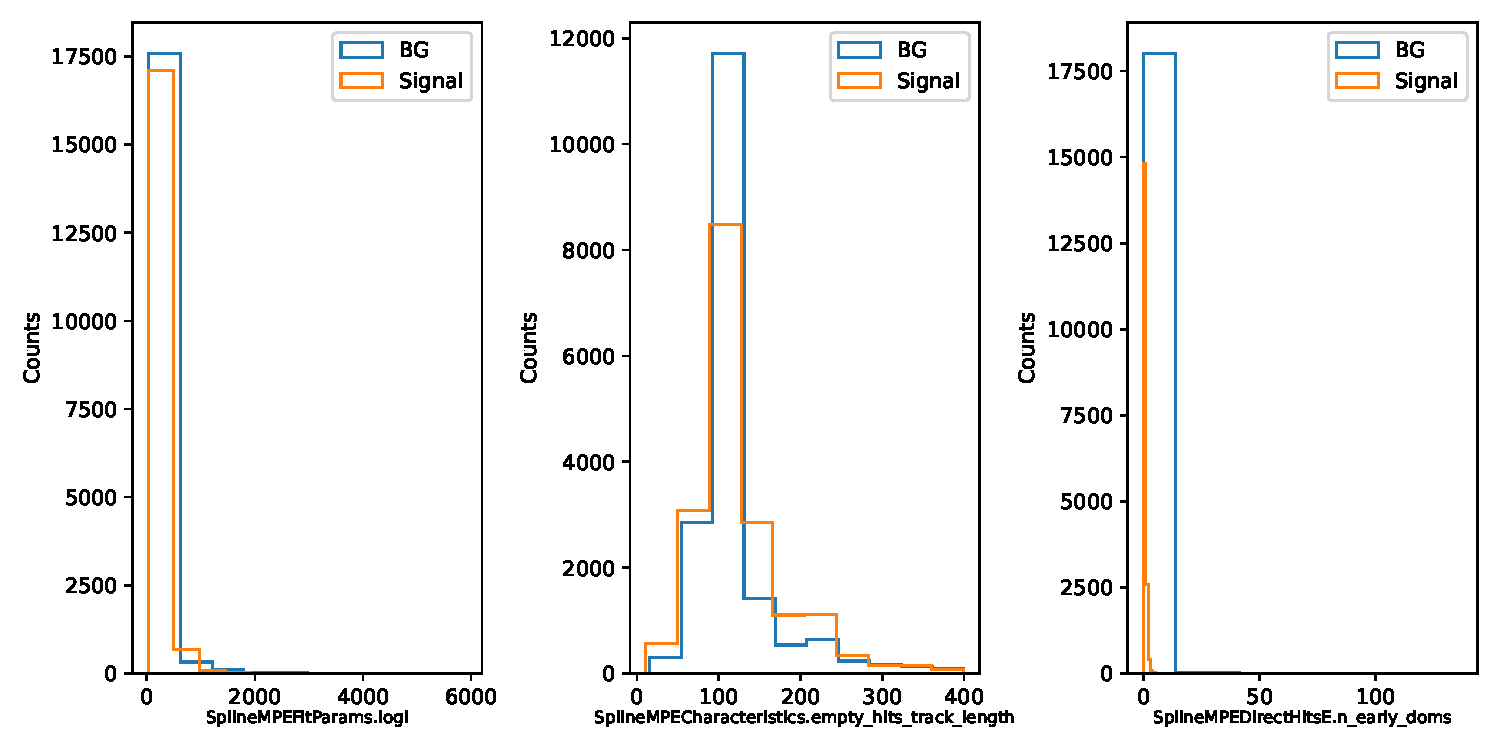
\includegraphics[width=0.9\textwidth]{content/plots/worst_3_features.pdf}
    \caption{The three worst features determined by an mRMR selection with a total of 100 features.}
    \label{fig:worst_features}
\end{figure}

\subsection{Multivariate selection}
The Naive Bayes, the Random Forest and the kNN classifiers are chosen for the multivariate selection. For all three classifiers, the ten best features are used and a k-fold with $n=\num{5}$ splits is performed. The classifiers are 
trained via the cross-validation method (see \autoref{sec:cross-validation}). A values of $\beta=0.1$ for the $f_{\beta}$ score (\eqref{eq:f_beta}) is used throughout this analysis, placing more importance on the precision rather 
than the recall. \\
The performance of each classifier is discussed in the following sections.

\subsubsection{Naives Bayes}
The working priciple of a Naive Bayes classifier is explained in \autoref{subsec:Bayes}. In \autoref{fig:apr_naive}, the accuracy, precision and recall metrics are portrayed.
\begin{figure}
    \centering
    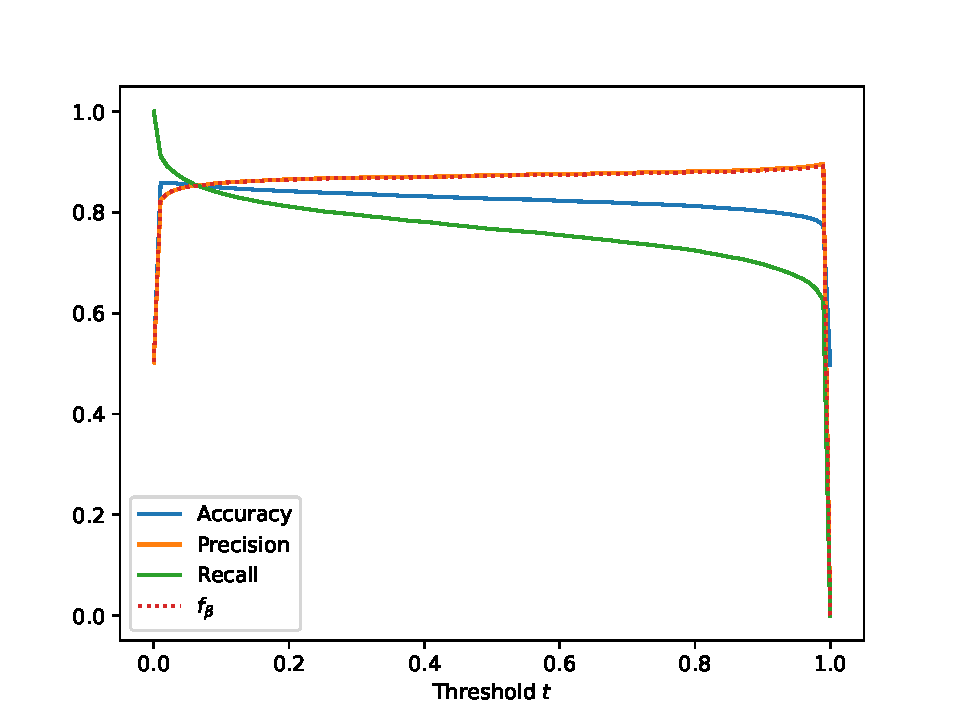
\includegraphics[width=0.7\textwidth]{content/plots/apr_naive.pdf}
    \caption{Naive Bayes: accuracy, precision and recall. Magnification of the relevant part of the $f_{\beta}$ score is shown in \autoref{fig:f_beta_naive}.} 
    \label{fig:apr_naive}
\end{figure}

\begin{figure}
    \centering
    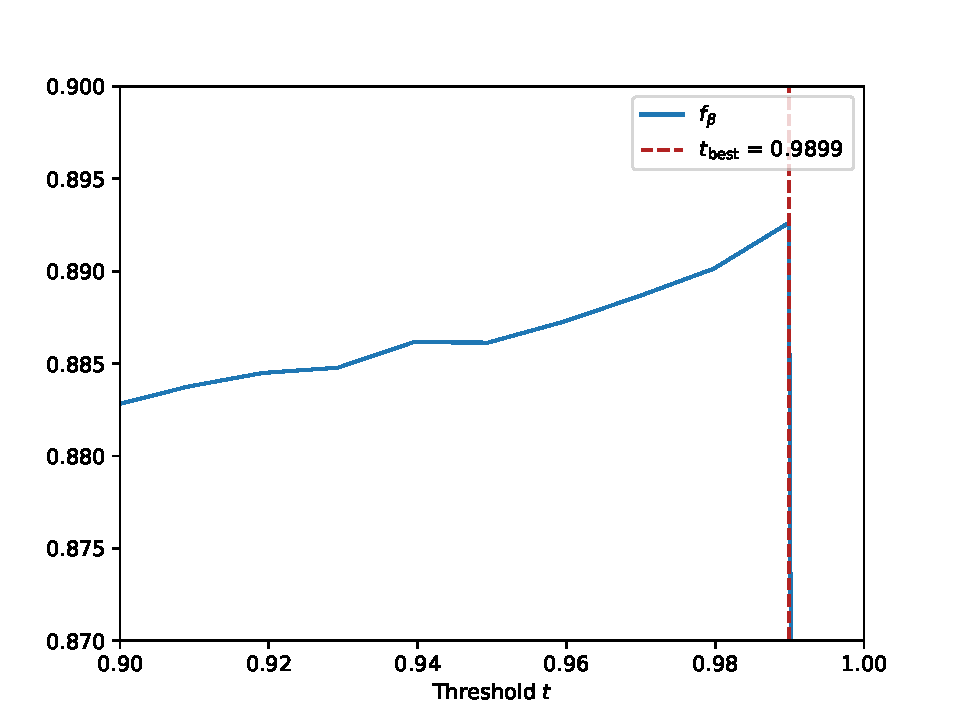
\includegraphics[width=0.7\textwidth]{content/plots/f_beta_naive.pdf}
    \caption{Naive Bayes: $f_{\beta}$ dependend on the threshold $t$. The maximum value for $f_{\beta}$ is marked with dashed lines.}
    \label{fig:f_beta_naive}
\end{figure}
The cross-validation of the Naive Bayes classifier yields the following quality parameters
% \begin{align*}
%     a &= \qty{0.827+-0.005} \\
%     p &= \qty{0.873+-0.006} \\
%     A_{\mathrm{ROC}} &= \qty{0.9211+-0.0033}.
% \end{align*}
\begin{align*}
    a &= \num{0.827 \pm 0.005} \\
    p &= \num{0.873 \pm 0.006} \\
    A_{\mathrm{ROC}} &= \num{0.9211 \pm 0.0033}
\end{align*}

The best value for the threshold $t$ is determined by finding the maximum of the $f_{\beta}$ score. This is depicted in \autoref{fig:f_beta_naive} and for the
Naive Bayes classifier an optimal threshold value of $t_{\mathrm{best}} = \num{0.9899}$ is obtained.
The confusion matrix of the classifier with this threshold value is shown in \autoref{fig:confusion_naive}.
\begin{figure}
    \centering
    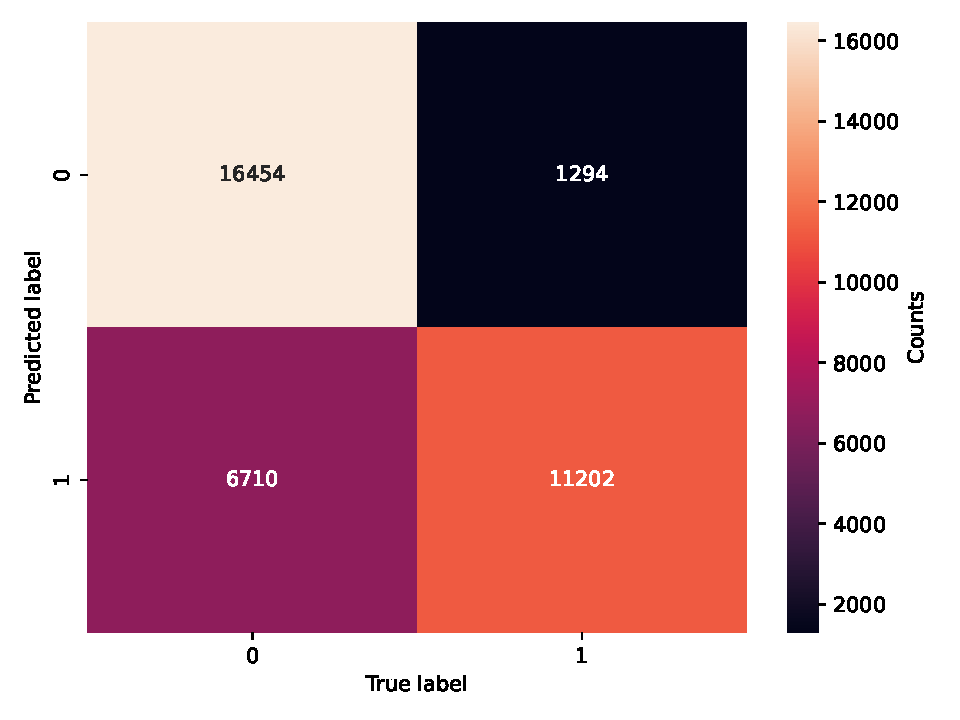
\includegraphics[width=0.7\textwidth]{content/plots/confusion_naive.pdf}
    \caption{Naive Bayes: Confusion matrix with threshold value $t_{\mathrm{best}} = \num{0.9899}$.}
    \label{fig:confusion_naive}
\end{figure}

\subsubsection{Random Forest}
As the second classifier, a Random Forest is selected. The idea behind decision trees is further addressed in \autoref{subsec:decision_trees}. Similar to the previous classifier,
a cross-validation is executed and the quality parameters are returned as
\begin{align*}
    a &= \num{0.9403(0.0019)} \\
    p &= \num{0.9544(0.0022)}  \\
    A_{\mathrm{ROC}} &= \num{0.9829(0.0012)}. \\
\end{align*}
For this classifier, the best threshold value is acquired as $t_{\mathrm{best}} = \num{0.8889}$. In the Figures \ref{fig:apr_rdm}, \ref{fig:f_beta_rdm} and \ref{fig:confusion_rdm}, the quality parameters
and the confusion matrix are shown.
\begin{figure}
    \centering
    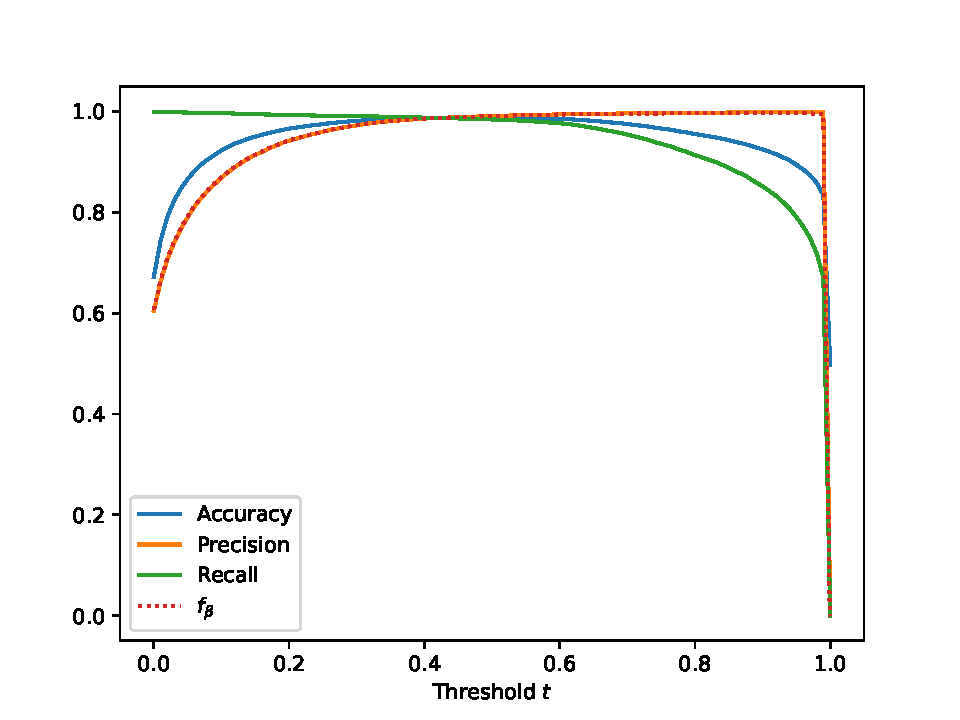
\includegraphics[width=0.7\textwidth]{content/plots/apr_rdm.pdf}
    \caption{Random Forest: accuracy, precision and recall. Magnification of the relevant part of the $f_{\beta}$ score is shown in \autoref{fig:f_beta_rdm}.}
    \label{fig:apr_rdm}
\end{figure}
\begin{figure}
    \centering
    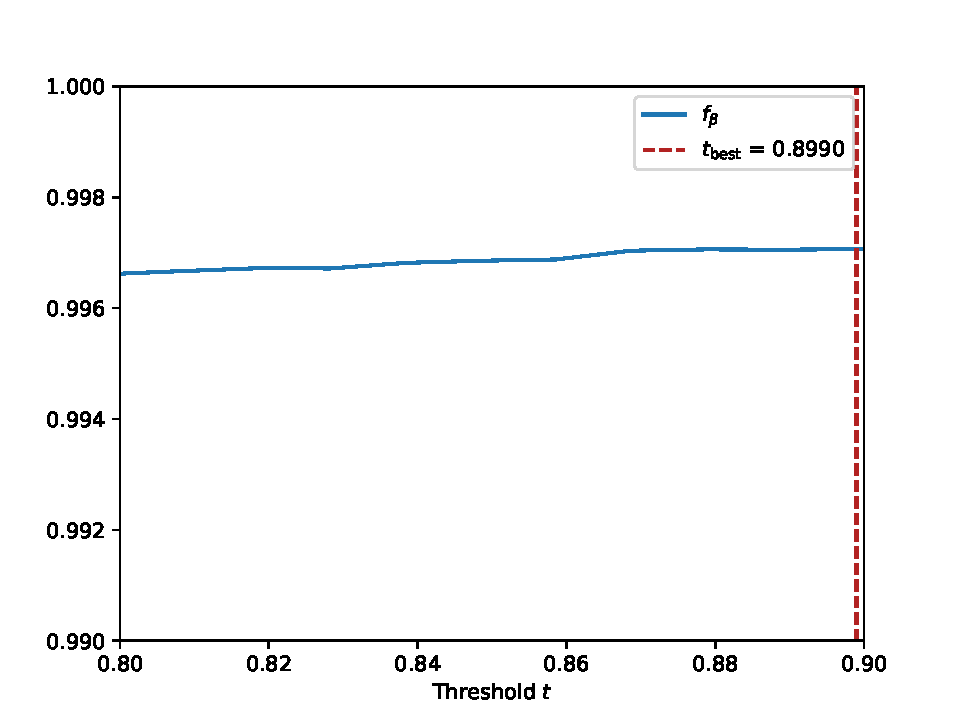
\includegraphics[width=0.7\textwidth]{content/plots/f_beta_rdm.pdf}
    \caption{Random Forest: $f_{\beta}$ dependend on the threshold $t$. The maximum value for $f_{\beta}$ is marked with dashed lines.}
    \label{fig:f_beta_rdm}
\end{figure}
\begin{figure}
    \centering
    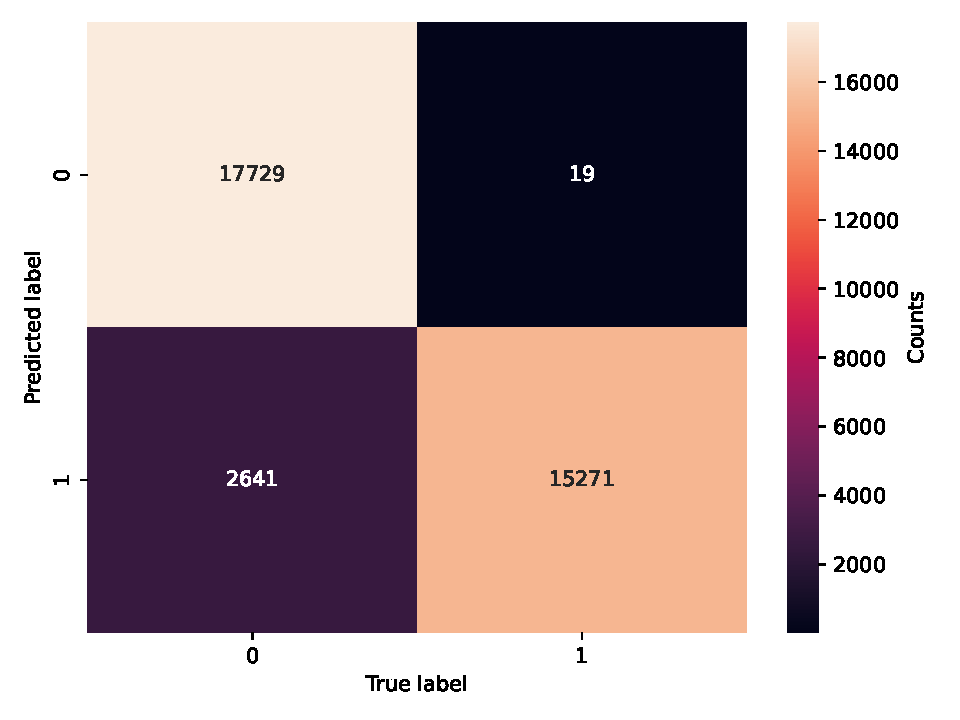
\includegraphics[width=0.7\textwidth]{content/plots/confusion_rdm.pdf}
    \caption{Random Forest: Confusion matrix with threshold value $t_{\mathrm{best}} = \num{0.8889}$.}
    \label{fig:confusion_rdm}
\end{figure}

\subsubsection{k nearest neighbors}
For the k nearest neighbors (kNN) algorithm, the procedure is the same as before. In \autoref{subsec:kNN}, this classifier is introduced.
The Figures \ref{fig:apr_kNN}, \ref{fig:f_beta_kNN} and \ref{fig:confusion_kNN} contain information about the quality parameters and the confusion 
matrix.

\begin{figure}
    \centering
    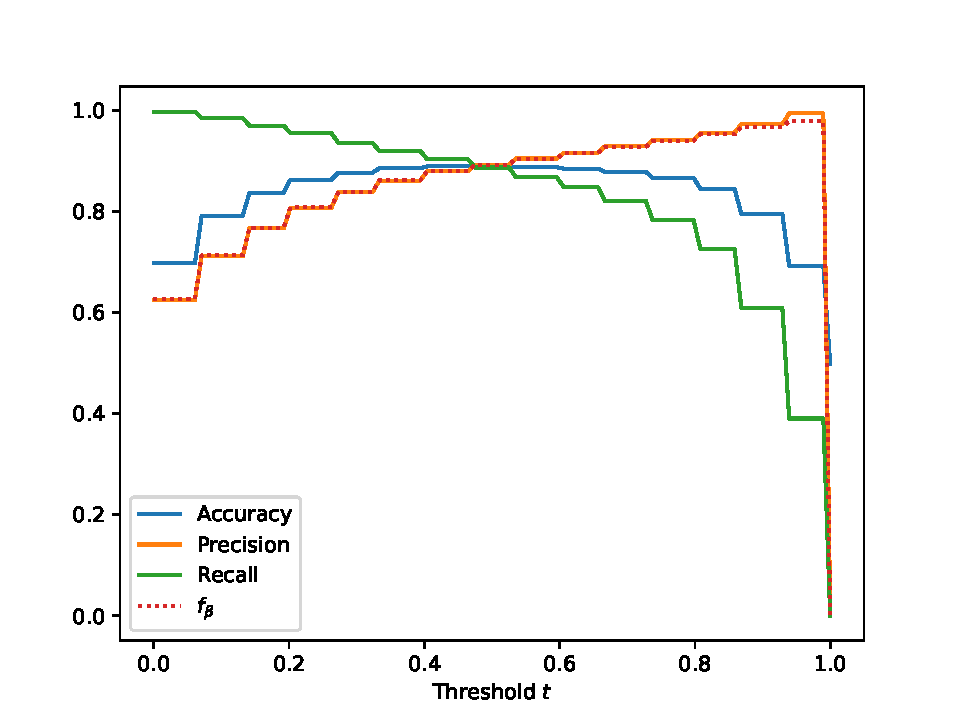
\includegraphics[width=0.7\textwidth]{content/plots/apr_kNN.pdf}
    \caption{kNN: accuracy, precision and recall. Magnification of the relevant part of the $f_{\beta}$ score is shown in \autoref{fig:f_beta_kNN}.}
    \label{fig:apr_kNN}
\end{figure}
\begin{figure}
    \centering
    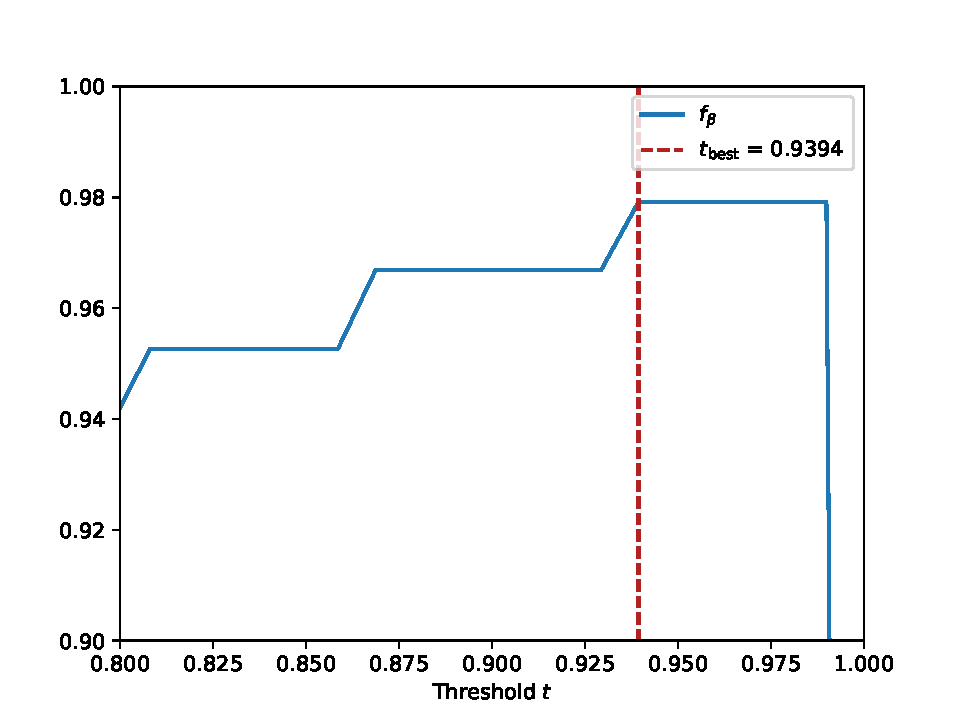
\includegraphics[width=0.7\textwidth]{content/plots/f_beta_kNN.pdf}
    \caption{kNN: $f_{\beta}$ dependend on the threshold $t$. The maximum value for $f_{\beta}$ is marked with dashed lines.}
    \label{fig:f_beta_kNN}
\end{figure}
\begin{figure}
    \centering
    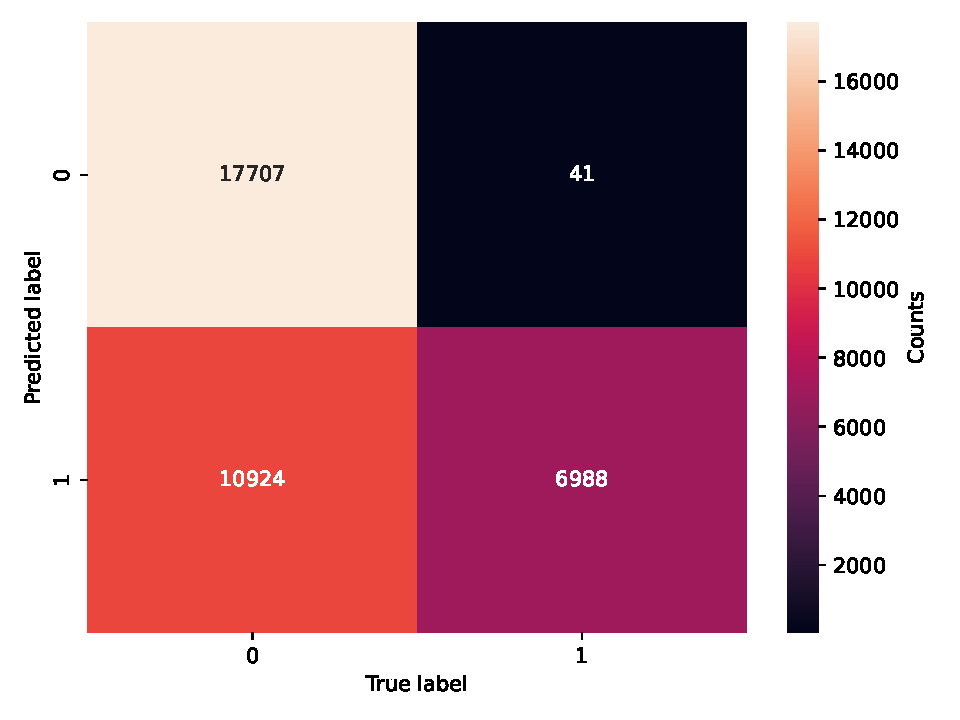
\includegraphics[width=0.7\textwidth]{content/plots/confusion_kNN.pdf}
    \caption{Random Forest: Confusion matrix with threshold value $t_{\mathrm{best}} = \num{0.9394}$.}
    \label{fig:confusion_kNN}
\end{figure}
The values for accuracy, precision, ROC-AUC score, and $f_{\beta}$ score are as follows
\begin{align*}
    a &= \num{0.8821+-0.0016} \\
    p &= \num{0.885+-0.007}  \\
    A_{\mathrm{ROC}} &= \num{0.9400+-0.0023} \\
    f_{\beta} &= \num{0.9394}.
\end{align*}

\subsection{Comparison of the learning algorithms}
In \autoref{fig:ROC_all}, the ROC curves for all three classifiers is depicted. The values for the true positive (TP) rate and the false positive (FP) rate are
extracted from the corresponding confusion matrices. The individual ROC-AUC scores are listed in \autoref{tab:ROC-AUC}.
\begin{figure}
    \centering
    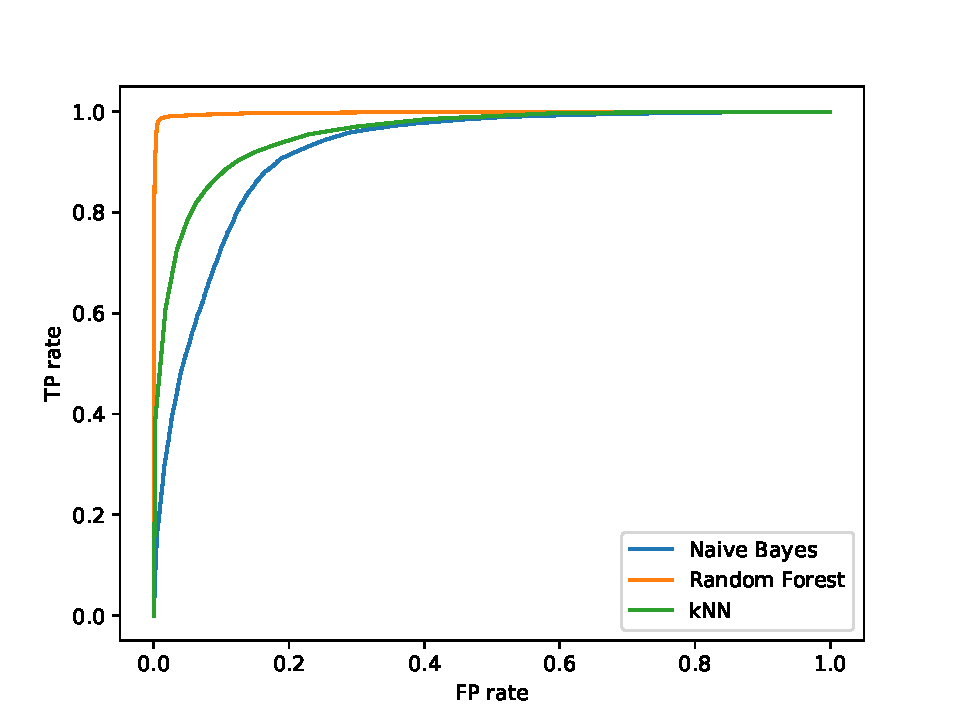
\includegraphics[width=0.7\textwidth]{content/plots/ROC_all.pdf}
    \caption{ROC curves for the three different classifiers.}
    \label{fig:ROC_all}
\end{figure}
\begin{table}
    \centering
    \caption{ROC-AUC scores for the different classifiers.}
    \label{tab:ROC-AUC}
      \begin{tabular}{c S}
        \toprule
        {Classifier} & {ROC-AUC score} \\
        \midrule
        {Naive Bayes}   & 0.9212 \\
        {Random Forest} & 0.9983 \\
        {kNN}           & 0.9562 \\
        \bottomrule 
      \end{tabular} 
  \end{table}

  The Random Forest classifier has been identified as the best-performing model and thus selected to classify the 
  provided \texttt{test.csv} dataset. Out of a total of 4000 events, 1633 are classified as signal, while the remaining 2367 
  are classified as background.
% \begin{figure}
%     \centering
%     \begin{subfigure}{0.49\textwidth}
%       \centering
%       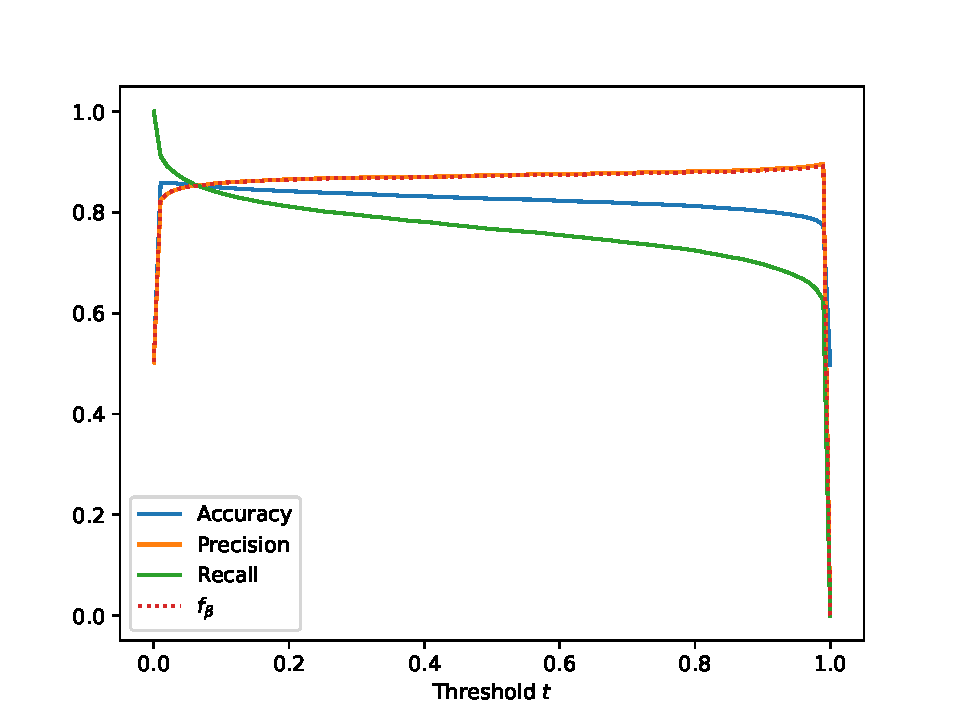
\includegraphics[width=\textwidth]{content/plots/apr_naive.pdf}
%       \caption{...}
%       \label{fig:roc_curve}
%     \end{subfigure}
%     % \hfill
%     \begin{subfigure}{0.49\textwidth}
%       \centering
%       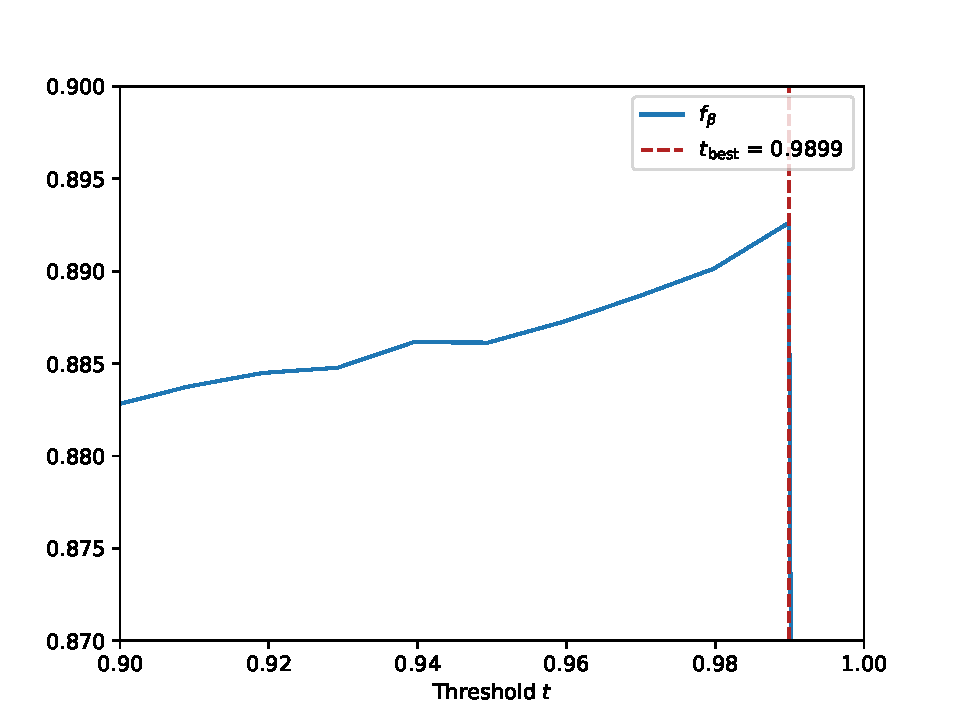
\includegraphics[width=\textwidth]{content/plots/f_beta_naive.pdf}
%       \caption{...}
%       \label{fig:train_test}
%     \end{subfigure}
%     \caption{...}
%     \label{fig:BDT}
%   \end{figure}
